
\documentclass[11pt,largemargins]{homework}
\usepackage{xcolor}
\usepackage{graphicx}

% TODO: replace these with your information
\newcommand{\hwname}{}
\newcommand{\hwemail}{}
\newcommand{\hwtype}{Big Pset}
\newcommand{\hwnum}{}
\newcommand{\hwclass}{AST 301}
\newcommand{\hwlecture}{}
\newcommand{\hwsection}{}

\begin{document}
\maketitle

\question
In frame $O$, a meter stick lies parallel to the $x$ axis and moves at velocity $V \mathbf{e}_y$.  Frame $\bar{O}$ is boosted relative to $O$ at velocity $\beta \mathbf{e}_x$ but not rotated, i.e., the spatial axes $\bar{x}\bar{y}\bar{z}$ lie parallel to $xyz$.  Show that in $\bar{O}$, the meter stick makes a nonzero angle $\theta$ with respect to the $\bar{x}$ axis, and derive an expression for $\theta$ in terms of $V$ and $\beta$. 

We use the relativistic velocity formulae, referencing Hartle (4.28), which assumes that as in our problem, the barred or primed frame is moving with some velocity in the $x$-drection.  Namely
\begin{subequations}
\begin{align}
V^{\bar{x}} &= \frac{V^{x} - v}{1 - v V^{x} / c^2}, \\
V^{\bar{y}} &= \frac{V^{y}}{1 - v V^{x} / c^2} \sqrt{1 - v^2 / c^2}.
\end{align}
\end{subequations}
Setting $c = 1$ and realizing $V^{x} = 0$, $V^{y} = V$, and $v = \beta$, we have
\begin{subequations}
\begin{align}
V^{\bar{x}} &= -\beta, \\
V^{\bar{y}} &= V \sqrt{1 - \beta^2}.
\end{align}
\end{subequations}
Recall that $\theta = \mathrm{arctan}(y / x)$, so 
\begin{equation}
\theta = \mathrm{arctan}(\frac{-V \sqrt{1 - \beta^2}}{\beta})
\end{equation}

\question
Observer $O$ constructs a clock in which a photon bounces back and forth along the $x$ axis at $x = 0$ and $x = L$. $O$ moves at speed $(4/5)c$ relative to $\bar{O}$ along the $x \bar{x}$ axis. 
\begin{alphaparts}

\questionpart
What is the round trip time between the two mirrors in frames $O$ and $\bar{O}$?
In frame $O$ the round trip time is simply the total distance $2L$ divided by $c$, i.e
\begin{equation}
\tau = \frac{2L}{c}
\end{equation}
To find the round trip time we use Hartle (4.15), which states
\begin{equation}
d\tau = d\bar{t} \sqrt{1 - V^2 / c^2}.
\end{equation}
For us, $d\tau = 2L/c$, so
\begin{subequations}
\begin{align*}
\frac{2L}{c} &= d\bar{t} \sqrt{1 - V^2 / c^2}, \\
d\bar{t} &= \frac{2L/c}{\sqrt{1 - V^2 / c^2}}, \\
d\bar{t} &= \frac{5}{3} \frac{2L}{c},
\end{align*}
\end{subequations}
Thus, the round trip time in $\bar{O}$ is
\begin{equation}
\bar{t} = \frac{10L}{c}
\end{equation}

\questionpart
What is the separation between the mirrors in $\bar{O}$?
Recall that 
\begin{equation}
\bar{L} = \frac{1}{\gamma} L_{0},
\end{equation}
where $L_{0}$ is the length in the rest frame.
Then
\begin{equation}
\bar{L} = \frac{3}{5} L
\end{equation}

\questionpart
The energy of the photon is $E$ in $O$.  What energy does $\bar{O}$ measure for the photon while it travels from $x = 0$ to $x = L$, and what energy does she measure while it travels from $x = L$ to $x = 0$?  (The mirrors are too massive to recoil appreciably.)

\begin{subequations}
\begin{align*}
E_{\mathrm{left}} &= \gamma \frac{E}{c} (1 + \beta) \\
&= \frac{1}{\sqrt{1 - (4/5)^2}} \frac{E}{c} (1 + 4/5) \\
&= \frac{3E}{c} \\ \\
E_{\mathrm{right}} &= \gamma \frac{E}{c} (1 - \beta) \\
&= \frac{1}{\sqrt{1 - (4/5)^2}} \frac{E}{c} (1 - 4/5) \\ 
&= \frac{E}{3c}
\end{align*}
\end{subequations}

\questionpart
If there are $N$ such photons distributed uniformly between the mirrors, all moving parallel to the $x$ axis, and with equal numbers moving in each direction as seen in $O$; and if the surface of each mirror is $A$, what are the components of the energy-momentum tensor due to these photons in frames $O$ and $\bar{O}$?

The energy momentum tensor $T$ is a rank 2 tensor, which means it can be represented by an ordinary matrix.  We have one spatial dimension and the time dimension, so it is represented by a $2 \times 2$ matrix.  Our strategy will be to find the components of $T$ in the frame $O$, and then use the Lorentz transform to find the components in $\bar{O}$. Then, in frame $O$: 

$T^{00}$ is the energy density, or the energy/volume.  So 
$$T^{00} = \frac{NE}{AL},$$ where E is the energy of each photon.  The $T^{10} = T^{01}$ components are the momentum density, which are zero.  The remaining component $T^{11}$ is the force per area in the x-direction.  (A full description of the energy-momentum tensor is in the appendix.) Then,
\begin{subequations}
\begin{align*}
T^{11} &= \frac{N}{2AL} \frac{E}{c} c + \frac{N}{2AL} \frac{-E}{c} (-c) \\
&= \frac{NE}{AL}
\end{align*}
\end{subequations}
Therefore, in $O$:

\begin{equation}
T = \frac{NE}{AL} \begin{pmatrix} 1 & 0 \\ 0 & 1 \end{pmatrix}
\end{equation}

To find the components of $T$ in $\bar{O}$, we perform a Lorentz transform.  Because we have two components for $T$, we have to do a matrix multiplication for each component.  The form of these matrix multiplications is
\begin{equation}
T^{\bar{\mu}\bar{\nu}} = \big[ \Lambda_{\nu}^{\bar{\nu}} \big]^{\top} T^{\mu \nu} \big[ \Lambda_{\mu}^{\bar{mu}} \big]
\end{equation}
Therefore, in $\bar{O}$

\begin{equation*}
T^{\bar{\mu} \bar{\nu}} = \frac{NE}{AL} \begin{pmatrix} \gamma & \gamma \beta \\ \gamma \beta & \gamma \end{pmatrix} \begin{pmatrix} 1 & 0 \\ 0 & 1 \end{pmatrix} \begin{pmatrix} \gamma & \gamma \beta \\ \gamma \beta & \gamma \end{pmatrix} 
\end{equation*}

\begin{equation}
T^{\bar{\mu} \bar{\nu}} = \frac{NE}{AL} \begin{pmatrix} \gamma^2 + \gamma^2 \beta^2 & 2 \gamma^2 \beta \\ 2 \gamma^2 \beta & \gamma^2 \beta^2 + \gamma^2 \end{pmatrix}
\end{equation}
\end{alphaparts}

\question An optical fiber of index of refraction $n > 1$ is bent into a circular ring of radius $r$ (much larger than the diameter of the fiber itself).  As seen from an inertial frame $O$, the ring rotates counterclockwise around its center at angular velocity $\Omega < c/r;$ the center of the ring is at rest in $O$.

\begin{alphaparts}
\questionpart
Calculate in frame $O$ the travel time of a light beam going once around the ring counterclockwise and returning to the same angular position as seen in $O$.  Let this be called $t_{+}$. 

\end{alphaparts}	
\setcounter{questionCounter}{10}

\question
Supermassive black holes reside in the center of most galaxies.  Every $10^4$ yr, typically a star approaches the black hole on a marginally bound, extremely eccentric orbit, with a pericenter $(r_p)$ small enough that the star is \textit{tidally disrupted} if the $\hat{r}\hat{r}$ component of the tidal field is $>GM_{*}/R_{*}^{3}$ where $M_*$ and $R_*$ are the mass and radius of the star.
\begin{alphaparts}
\questionpart
Estimate the maximum $r_p$ for tidal disruption of the Sun in terms of $M_{\mathrm{bh}}$.  $M_{\odot} \approx 2 x 10^{33} \mathrm{g}$, $R_{\odot} \approx 7 x 10^{10} \mathrm{cm}$

Outside a spherical mass of $M_{\mathrm{bh}}$,
\begin{equation}
a_{\hat{r}\hat{r}} = \frac{2M_{\mathrm{bh}}}{r_{p}^{3}},
\end{equation}
according to Hartle (21.8). ($G = 1$ units).  The limit we are concerned with is $a_{\hat{r}\hat{r}} > GM_{*}/R_{*}^{3}$, so we set 
\begin{equation}
\frac{2M_{\mathrm{bh}}}{r_{p}^{3}} = \frac{G M_{*}}{R_{*}^{3}},
\end{equation} 
and solve for $r_{p}$, which yields
\begin{equation}
r_{p} = \bigg(\frac{2 M_\mathrm{bh}}{M_{\odot}} \bigg) ^ {1/3} R_{\odot}
\end{equation}

\questionpart
Just as disrupted/evaporated comets make meteor streams, the debris of a disrupted
star will spread out along the star?s original orbit. However, this leads to
observable consequences only if that orbit does not plunge into the black hole. Estimate the maximum black-hole mass for which a sunlike star can be disrupted on a
non-plunging, marginally-bound orbit.

Our limit for the Innermost Stable Circular Orbit (ISCO) is given by 

\begin{equation}
r_{c} = 6M_{\mathrm{bh}}
\end{equation}
in $G = 1$ units.  (Hartle 9.43 and derived in the lecture 12 slides).  Note that whenever we redimensionalize from mass to radius we simply multiply the mass by a factor of $G/c^2$.  (You can check these units!)

In order to disrupt the star in the non-plunging orbit, we must have $r_{c} > r_{p}$, so to investigate the limiting behavior, we simply set $r_{c} = r_{p}$.  Then we have

\begin{subequations}
\begin{align}
\frac{6 G M_\mathrm{bh}}{c^2} &= \bigg(\frac{2 M_\mathrm{bh}}{M_{\odot}} \bigg) ^ {1/3} R_{\odot} \\
\frac{6G}{2^{1/3}} \frac{M_{\mathrm{bh}}^{2/3}}{c^2} &= R_{\odot} M_{\odot}^{-1/3} \\
M_{\mathrm{bh}} &= \frac{c^3 \sqrt{2}}{6 G^{3/2}} R_{\odot}^{3/2} M_{\odot}^{-1/2}
\end{align}
\end{subequations}
Which we can evaluate for $M_{\mathrm{bh}}$.  Wolfram says it is on the order of $7 x 10^{7} M_{\odot}$.  

\questionpart

Assuming $r_p \gg M$, estimate the radius $r_i \gg r_p$ at which the outgoing part of the orbit intersects the incoming part.  You may use the following approximation for the change in periapse angle per period of a nearly keplerian ($r_p \gg M$) orbit of semi-major axis $a$ and eccentricity $\epsilon:$

\begin{equation}
\delta \phi_{p} \approx \frac{6 \pi M}{a(1 - \epsilon^2)}
\end{equation}

and recall $r_{p} = a(1 - \epsilon)$ and $r(\phi) = a(1 - \epsilon^2) / [1 + \epsilon \cos{(\phi - \phi_{p}})]$.

It's a little tricky to visualize what is going on in this problem, so I've included a figure.  $r_i$ is the intersection between the two ellipses formed here. 
\begin{figure}[h]
\centering
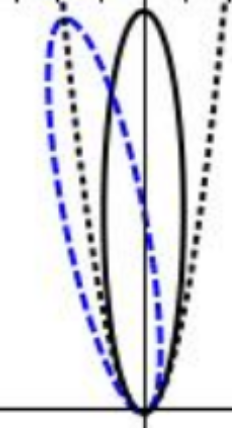
\includegraphics[scale=0.6]{orbits}
\caption{$r_{i}$ is the intersection of the two ellipses.}
\end{figure}

Let's be clear about what this means. The two ellipses are both defined by the equation $r(\phi)$.  The only difference between the two is the argument of the periapsis, $\phi_{p}$.  In order for the two ellipses to intersect, we require:

\begin{equation}
\frac{a(1 - \epsilon^2)}{1 + \epsilon \cos(\phi - \phi_{p})} = \frac{a(1 - \epsilon^2)}{1+\epsilon \cos(\phi - \phi_{p} - \delta \phi_{p})}
\end{equation}

But all this means is that $\cos(\phi - \phi_{p}) - \cos(\phi - \phi_{p} - \delta \phi_{p})$. This seems like it would be really ugly to solve, until we remember that $\cos(x)$ has some nice properties, specifically, that it is even and periodic.  Let $\phi = \delta \phi_{p} / 2$, and notice that we get

$$
\cos{(\delta \phi_{p}/2 - \phi_{p})} = \cos(-\phi_{p} - \delta \phi_{p} / 2) = \cos(\delta \phi_{p} / 2 - \phi_{p} - \delta \phi_{p}) 
$$

Now we can plug $\phi$ back into $r(\phi)$ and solve for $r_{i}$.  Doing so, we obtain:

\begin{equation}
r_{i} = \frac{r_{p} (1 + \epsilon)}{1 + \epsilon \cos(3 \pi M/ a(1 - \epsilon^2))}
\end{equation}
\end{alphaparts}
\end{document}